%%%%%%%%%%%%%%%%%%%%%%%%%%%%%%%%%%%%%%%%%
% fphw Assignment
% LaTeX Template
% Version 1.0 (27/04/2019)
%
% This template originates from:
% https://www.LaTeXTemplates.com
%
% Authors:
% Class by Felipe Portales-Oliva (f.portales.oliva@gmail.com) with template 
% content and modifications by Vel (vel@LaTeXTemplates.com)
%
% Template (this file) License:
% CC BY-NC-SA 3.0 (http://creativecommons.org/licenses/by-nc-sa/3.0/)
%
%%%%%%%%%%%%%%%%%%%%%%%%%%%%%%%%%%%%%%%%%

%----------------------------------------------------------------------------------------
%	PACKAGES AND OTHER DOCUMENT CONFIGURATIONS
%----------------------------------------------------------------------------------------

\documentclass[
	12pt, % Default font size, values between 10pt-12pt are allowed
	%letterpaper, % Uncomment for US letter paper size
	%spanish, % Uncomment for Spanish
]{../Template/fphw}

% Template-specific packages
\usepackage[utf8]{inputenc} % Required for inputting international characters
\usepackage[T1]{fontenc} % Output font encoding for international characters
\usepackage{mathpazo} % Use the Palatino font

\usepackage{graphicx} % Required for including images

\usepackage{booktabs} % Required for better horizontal rules in tables

\usepackage{listings} % Required for insertion of code

\usepackage{enumerate} % To modify the enumerate environment

% Additional packages needed
\usepackage{amsmath}
\usepackage{enumitem}
\usepackage{mwe}
\usepackage{comment}
\usepackage{url}
\usepackage{algorithm}
\usepackage{algpseudocode}
\usepackage{tikz}

%----------------------------------------------------------------------------------------
%	ASSIGNMENT INFORMATION
%----------------------------------------------------------------------------------------

\title{Programming Project \#1} % Assignment title

\author{Mao Nishino, Farez Siddiqui} % Student name

\date{March 19th, 2024} % Due date

\institute{Florida State University \\ Department of Computer Science} % Institute or school name

\class{Deep and Reinforcement Learning Fundamentals (CAP5619-0001.sp24)} % Course or class name

\professor{Dr. Xiuwen Liu} % Professor or teacher in charge of the assignment

%----------------------------------------------------------------------------------------

\begin{document}

\maketitle % Output, the assignment title, created automatically using the information in the custom commands above

%----------------------------------------------------------------------------------------
%	ASSIGNMENT CONTENT
%----------------------------------------------------------------------------------------

\section*{Task I - Neural Network Design}

\begin{problem}
In the deep learning framework you have set up, design three different neural networks. Each one must have
at least four layers; rectified activation functions must be used at least in one of the layers (among all the
three networks) and sigmoid/tanh activation functions must be used in one of the layers as well (among
all the three networks). The overall connection requirements are as follows:
\begin{enumerate}[label = (\arabic*)]
\item Fully connected, where each input/neuron is connected to all the neurons in the next layer
\item Locally connected with no weights shared in the first three layers, where each input/neuron is
connected to the neurons in a local neighbor in the next layer
\item Locally connected with weights shared in the first three layers (i.e., a convolutional neural network)
\end{enumerate}
In your report, you need to provide explanations of your design choices and describe your neural networks clearly.
\end{problem}

%------------------------------------------------

\subsection*{Answer}
The architectures for each network are shown in Figure \ref{fig:p1_architectures}. We will give detailed descriptions and explanations behind the design choices.
\begin{enumerate}[label = (\arabic*)] 
	\item This is a fully connected four-layer neural network with ReLU as activation functions.  We have chosen ReLU as the activation function because this is the standard default choice \cite[p188]{Goodfellow-et-al-2016} and other choices such as the sigmoidal function or tanh are discouraged for saturation issues when used in hidden layers\cite[p191]{Goodfellow-et-al-2016}. As for the number of layers, we have chosen $4$ simply because it was the minimal number we were required to have.  
 
    \textbf{Extra Credit Attempt: Architecture Optimization} We have employed the commonly used "coarse-to-fine" strategy to choose the number of neurons in each layer. The detailed algorithm is stated in Algorithm \ref{alg:NAS}. We have predetermined any hyperparameters other than the number of neurons for simplicity and ease of training. Still, the idea of the algorithm is clearly applicable in more general search spaces. The basic idea of the algorithm is to conduct random searches in increasingly smaller search spaces. Although there are other search strategies, such as reinforcement learning-based or evolutionary algorithm-based algorithms \cite[p68]{automl}, we have chosen a random search-based algorithm because it is simple to implement. Although random search performs worse than the aforementioned methods, the gain from choosing them is often small \cite[p69]{automl}. To alleviate the computational cost, we start from the models trained with less training time. We gradually increase the training time by increasing the number of epochs and decreasing the batch size. That is, we take a common strategy of evaluating performance in less complicated situations and gradually increasing complexity for more accurate performance estimation, as recommended in \cite[p71]{automl}.
    
	\item Since this is the convolutional network without weight sharing, we have replaced the convolution layers in the convolutional network we introduce later with locally connected layers. As \verb|PyTorch|\cite{pytorch} does not have locally connected layers implemented, we have implemented ourselves, and the implementation details can be found in our notebook. Moreover, to satisfy the requirement to have a sigmoidal activation function somewhere, we used it for our output layer. As mentioned, we avoided using it in hidden layers due to the saturation issue.

    \item As our starting point, we have looked at one of the earliest papers on the convolutional network \cite{convnet_original}, which also works on the same data as ours. Their architecture already boasts a test error rate of 3.4\%, but the choice of layers is outdated in the current standard. So, we have taken their architecture and modernized the design, following the recommendations in \cite{Goodfellow-et-al-2016}. (write more about details, citing the textbook)
    
\end{enumerate}


\begin{figure}[!htbp]
    \centering

    





\tikzset{every picture/.style={line width=0.75pt}} %set default line width to 0.75pt        

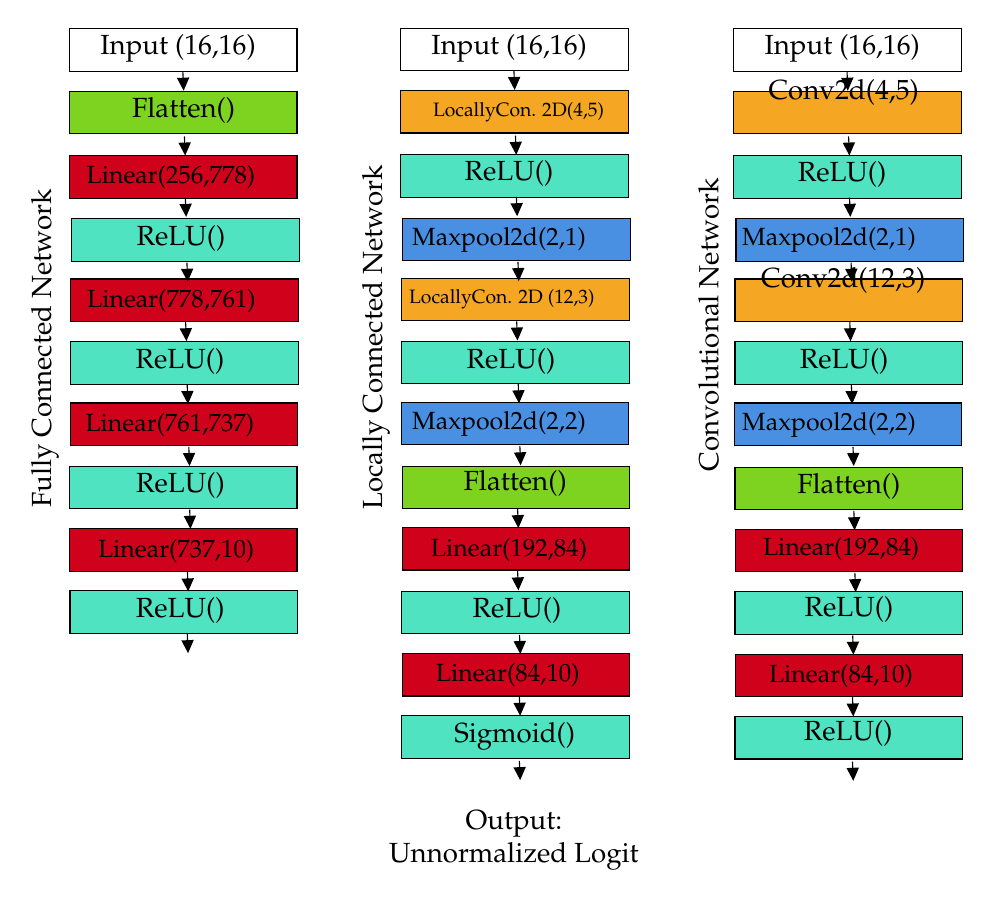
\begin{tikzpicture}[x=0.75pt,y=0.75pt,yscale=-1,xscale=1]
%uncomment if require: \path (0,461); %set diagram left start at 0, and has height of 461

%Flowchart: Process [id:dp02351632173585183] 
\draw  [fill={rgb, 255:red, 255; green, 255; blue, 255 }  ,fill opacity=1 ] (112.25,11.5) -- (221.75,11.5) -- (221.75,32) -- (112.25,32) -- cycle ;
%Flowchart: Process [id:dp42941465319220407] 
\draw  [fill={rgb, 255:red, 126; green, 211; blue, 33 }  ,fill opacity=1 ] (112.25,41.5) -- (221.75,41.5) -- (221.75,62) -- (112.25,62) -- cycle ;
%Flowchart: Process [id:dp08453394336733022] 
\draw  [fill={rgb, 255:red, 208; green, 2; blue, 27 }  ,fill opacity=1 ] (112.25,72.5) -- (221.75,72.5) -- (221.75,93) -- (112.25,93) -- cycle ;
%Flowchart: Process [id:dp4778014521769103] 
\draw  [fill={rgb, 255:red, 80; green, 227; blue, 194 }  ,fill opacity=1 ] (113.25,103) -- (222.75,103) -- (222.75,123.5) -- (113.25,123.5) -- cycle ;
%Flowchart: Process [id:dp9306397015209844] 
\draw  [fill={rgb, 255:red, 208; green, 2; blue, 27 }  ,fill opacity=1 ] (112.75,132) -- (222.25,132) -- (222.25,152.5) -- (112.75,152.5) -- cycle ;
%Flowchart: Process [id:dp9050309774198928] 
\draw  [fill={rgb, 255:red, 80; green, 227; blue, 194 }  ,fill opacity=1 ] (112.75,162.25) -- (222.25,162.25) -- (222.25,182.75) -- (112.75,182.75) -- cycle ;
%Flowchart: Process [id:dp6677905436834566] 
\draw  [fill={rgb, 255:red, 208; green, 2; blue, 27 }  ,fill opacity=1 ] (112.5,191.75) -- (222,191.75) -- (222,212.25) -- (112.5,212.25) -- cycle ;
%Flowchart: Process [id:dp05592789910796103] 
\draw  [fill={rgb, 255:red, 80; green, 227; blue, 194 }  ,fill opacity=1 ] (112.25,222.25) -- (221.75,222.25) -- (221.75,242.75) -- (112.25,242.75) -- cycle ;
%Flowchart: Process [id:dp9952366943934081] 
\draw  [fill={rgb, 255:red, 208; green, 2; blue, 27 }  ,fill opacity=1 ] (112.25,252.25) -- (221.75,252.25) -- (221.75,272.75) -- (112.25,272.75) -- cycle ;
%Flowchart: Process [id:dp8718199900480916] 
\draw  [fill={rgb, 255:red, 80; green, 227; blue, 194 }  ,fill opacity=1 ] (112.4,282.25) -- (221.9,282.25) -- (221.9,302.75) -- (112.4,302.75) -- cycle ;
%Straight Lines [id:da9533929994486752] 
\draw    (166.75,32) -- (167,38.25) ;
\draw [shift={(167.13,41.25)}, rotate = 267.68] [fill={rgb, 255:red, 0; green, 0; blue, 0 }  ][line width=0.08]  [draw opacity=0] (6.25,-3) -- (0,0) -- (6.25,3) -- cycle    ;
%Straight Lines [id:da28583644695644894] 
\draw    (167.5,63.25) -- (167.75,69.5) ;
\draw [shift={(167.88,72.5)}, rotate = 267.68] [fill={rgb, 255:red, 0; green, 0; blue, 0 }  ][line width=0.08]  [draw opacity=0] (6.25,-3) -- (0,0) -- (6.25,3) -- cycle    ;
%Straight Lines [id:da03204029710574252] 
\draw    (167.95,92.8) -- (168.2,99.05) ;
\draw [shift={(168.33,102.05)}, rotate = 267.68] [fill={rgb, 255:red, 0; green, 0; blue, 0 }  ][line width=0.08]  [draw opacity=0] (6.25,-3) -- (0,0) -- (6.25,3) -- cycle    ;
%Straight Lines [id:da7872545420609312] 
\draw    (168.7,124.05) -- (168.95,130.3) ;
\draw [shift={(169.08,133.3)}, rotate = 267.68] [fill={rgb, 255:red, 0; green, 0; blue, 0 }  ][line width=0.08]  [draw opacity=0] (6.25,-3) -- (0,0) -- (6.25,3) -- cycle    ;
%Straight Lines [id:da32793245802759863] 
\draw    (168.88,303) -- (169.14,309.25) ;
\draw [shift={(169.26,312.25)}, rotate = 267.68] [fill={rgb, 255:red, 0; green, 0; blue, 0 }  ][line width=0.08]  [draw opacity=0] (6.25,-3) -- (0,0) -- (6.25,3) -- cycle    ;
%Straight Lines [id:da8267605040931463] 
\draw    (168.97,273.25) -- (169.22,279.5) ;
\draw [shift={(169.34,282.5)}, rotate = 267.68] [fill={rgb, 255:red, 0; green, 0; blue, 0 }  ][line width=0.08]  [draw opacity=0] (6.25,-3) -- (0,0) -- (6.25,3) -- cycle    ;
%Straight Lines [id:da9742587362750603] 
\draw    (168.08,152.7) -- (168.34,158.95) ;
\draw [shift={(168.46,161.95)}, rotate = 267.68] [fill={rgb, 255:red, 0; green, 0; blue, 0 }  ][line width=0.08]  [draw opacity=0] (6.25,-3) -- (0,0) -- (6.25,3) -- cycle    ;
%Straight Lines [id:da008937420928793793] 
\draw    (168.83,182.95) -- (169.09,189.2) ;
\draw [shift={(169.21,192.2)}, rotate = 267.68] [fill={rgb, 255:red, 0; green, 0; blue, 0 }  ][line width=0.08]  [draw opacity=0] (6.25,-3) -- (0,0) -- (6.25,3) -- cycle    ;
%Straight Lines [id:da10562370725328729] 
\draw    (169.62,212.83) -- (169.87,219.09) ;
\draw [shift={(169.99,222.08)}, rotate = 267.68] [fill={rgb, 255:red, 0; green, 0; blue, 0 }  ][line width=0.08]  [draw opacity=0] (6.25,-3) -- (0,0) -- (6.25,3) -- cycle    ;
%Straight Lines [id:da5036344051727422] 
\draw    (170.03,243.08) -- (170.29,249.34) ;
\draw [shift={(170.41,252.33)}, rotate = 267.68] [fill={rgb, 255:red, 0; green, 0; blue, 0 }  ][line width=0.08]  [draw opacity=0] (6.25,-3) -- (0,0) -- (6.25,3) -- cycle    ;
%Flowchart: Process [id:dp07654239667008067] 
\draw  [fill={rgb, 255:red, 255; green, 255; blue, 255 }  ,fill opacity=1 ] (271.75,11.17) -- (381.25,11.17) -- (381.25,31.67) -- (271.75,31.67) -- cycle ;
%Flowchart: Process [id:dp37376964215801745] 
\draw  [fill={rgb, 255:red, 245; green, 166; blue, 35 }  ,fill opacity=1 ] (271.75,41.17) -- (381.25,41.17) -- (381.25,61.67) -- (271.75,61.67) -- cycle ;
%Flowchart: Process [id:dp3428413998103992] 
\draw  [fill={rgb, 255:red, 80; green, 227; blue, 194 }  ,fill opacity=1 ] (271.75,72.17) -- (381.25,72.17) -- (381.25,92.67) -- (271.75,92.67) -- cycle ;
%Flowchart: Process [id:dp629266102559507] 
\draw  [fill={rgb, 255:red, 74; green, 144; blue, 226 }  ,fill opacity=1 ] (272.75,102.67) -- (382.25,102.67) -- (382.25,123.17) -- (272.75,123.17) -- cycle ;
%Flowchart: Process [id:dp7074374276144555] 
\draw  [fill={rgb, 255:red, 245; green, 166; blue, 35 }  ,fill opacity=1 ] (272.25,131.67) -- (381.75,131.67) -- (381.75,152.17) -- (272.25,152.17) -- cycle ;
%Flowchart: Process [id:dp15281786912615014] 
\draw  [fill={rgb, 255:red, 80; green, 227; blue, 194 }  ,fill opacity=1 ] (272.25,161.92) -- (381.75,161.92) -- (381.75,182.42) -- (272.25,182.42) -- cycle ;
%Flowchart: Process [id:dp556820525114857] 
\draw  [fill={rgb, 255:red, 74; green, 144; blue, 226 }  ,fill opacity=1 ] (272,191.42) -- (381.5,191.42) -- (381.5,211.92) -- (272,211.92) -- cycle ;
%Flowchart: Process [id:dp6854555639120627] 
\draw  [fill={rgb, 255:red, 208; green, 2; blue, 27 }  ,fill opacity=1 ] (272.5,251.67) -- (382,251.67) -- (382,272.17) -- (272.5,272.17) -- cycle ;
%Flowchart: Process [id:dp34589582378519923] 
\draw  [fill={rgb, 255:red, 80; green, 227; blue, 194 }  ,fill opacity=1 ] (272.25,282.42) -- (381.75,282.42) -- (381.75,302.92) -- (272.25,302.92) -- cycle ;
%Flowchart: Process [id:dp4199329151131661] 
\draw  [fill={rgb, 255:red, 208; green, 2; blue, 27 }  ,fill opacity=1 ] (272.4,312.42) -- (381.9,312.42) -- (381.9,332.92) -- (272.4,332.92) -- cycle ;
%Straight Lines [id:da29287117438362475] 
\draw    (326.25,31.67) -- (326.5,37.92) ;
\draw [shift={(326.63,40.92)}, rotate = 267.68] [fill={rgb, 255:red, 0; green, 0; blue, 0 }  ][line width=0.08]  [draw opacity=0] (6.25,-3) -- (0,0) -- (6.25,3) -- cycle    ;
%Straight Lines [id:da8715728513895342] 
\draw    (327,62.92) -- (327.25,69.17) ;
\draw [shift={(327.38,72.17)}, rotate = 267.68] [fill={rgb, 255:red, 0; green, 0; blue, 0 }  ][line width=0.08]  [draw opacity=0] (6.25,-3) -- (0,0) -- (6.25,3) -- cycle    ;
%Straight Lines [id:da2767853528454396] 
\draw    (327.45,92.47) -- (327.7,98.72) ;
\draw [shift={(327.83,101.72)}, rotate = 267.68] [fill={rgb, 255:red, 0; green, 0; blue, 0 }  ][line width=0.08]  [draw opacity=0] (6.25,-3) -- (0,0) -- (6.25,3) -- cycle    ;
%Straight Lines [id:da9139221237028485] 
\draw    (328.2,123.72) -- (328.45,129.97) ;
\draw [shift={(328.58,132.97)}, rotate = 267.68] [fill={rgb, 255:red, 0; green, 0; blue, 0 }  ][line width=0.08]  [draw opacity=0] (6.25,-3) -- (0,0) -- (6.25,3) -- cycle    ;
%Straight Lines [id:da334115025888331] 
\draw    (328.88,333.17) -- (329.14,339.42) ;
\draw [shift={(329.26,342.42)}, rotate = 267.68] [fill={rgb, 255:red, 0; green, 0; blue, 0 }  ][line width=0.08]  [draw opacity=0] (6.25,-3) -- (0,0) -- (6.25,3) -- cycle    ;
%Straight Lines [id:da623702185150133] 
\draw    (328.97,303.42) -- (329.22,309.67) ;
\draw [shift={(329.34,312.67)}, rotate = 267.68] [fill={rgb, 255:red, 0; green, 0; blue, 0 }  ][line width=0.08]  [draw opacity=0] (6.25,-3) -- (0,0) -- (6.25,3) -- cycle    ;
%Straight Lines [id:da12298939627023597] 
\draw    (327.58,152.37) -- (327.84,158.62) ;
\draw [shift={(327.96,161.62)}, rotate = 267.68] [fill={rgb, 255:red, 0; green, 0; blue, 0 }  ][line width=0.08]  [draw opacity=0] (6.25,-3) -- (0,0) -- (6.25,3) -- cycle    ;
%Straight Lines [id:da8763601037493007] 
\draw    (328.33,182.62) -- (328.59,188.87) ;
\draw [shift={(328.71,191.87)}, rotate = 267.68] [fill={rgb, 255:red, 0; green, 0; blue, 0 }  ][line width=0.08]  [draw opacity=0] (6.25,-3) -- (0,0) -- (6.25,3) -- cycle    ;
%Straight Lines [id:da6421658225619669] 
\draw    (329.12,212.5) -- (329.37,218.75) ;
\draw [shift={(329.49,221.75)}, rotate = 267.68] [fill={rgb, 255:red, 0; green, 0; blue, 0 }  ][line width=0.08]  [draw opacity=0] (6.25,-3) -- (0,0) -- (6.25,3) -- cycle    ;
%Straight Lines [id:da35909666112314986] 
\draw    (328.03,272.75) -- (328.29,279) ;
\draw [shift={(328.41,282)}, rotate = 267.68] [fill={rgb, 255:red, 0; green, 0; blue, 0 }  ][line width=0.08]  [draw opacity=0] (6.25,-3) -- (0,0) -- (6.25,3) -- cycle    ;
%Flowchart: Process [id:dp49794632990715604] 
\draw  [fill={rgb, 255:red, 80; green, 227; blue, 194 }  ,fill opacity=1 ] (272.25,342.42) -- (381.75,342.42) -- (381.75,362.92) -- (272.25,362.92) -- cycle ;
%Straight Lines [id:da26795199376819423] 
\draw    (328.88,364.17) -- (329.14,370.42) ;
\draw [shift={(329.26,373.42)}, rotate = 267.68] [fill={rgb, 255:red, 0; green, 0; blue, 0 }  ][line width=0.08]  [draw opacity=0] (6.25,-3) -- (0,0) -- (6.25,3) -- cycle    ;
%Flowchart: Process [id:dp5682047520026112] 
\draw  [fill={rgb, 255:red, 255; green, 255; blue, 255 }  ,fill opacity=1 ] (432.25,11.5) -- (541.75,11.5) -- (541.75,32) -- (432.25,32) -- cycle ;
%Flowchart: Process [id:dp6597728419761311] 
\draw  [fill={rgb, 255:red, 245; green, 166; blue, 35 }  ,fill opacity=1 ] (432.25,41.5) -- (541.75,41.5) -- (541.75,62) -- (432.25,62) -- cycle ;
%Flowchart: Process [id:dp8809875064098089] 
\draw  [fill={rgb, 255:red, 80; green, 227; blue, 194 }  ,fill opacity=1 ] (432.25,72.5) -- (541.75,72.5) -- (541.75,93) -- (432.25,93) -- cycle ;
%Flowchart: Process [id:dp985728348238234] 
\draw  [fill={rgb, 255:red, 74; green, 144; blue, 226 }  ,fill opacity=1 ] (433.25,103) -- (542.75,103) -- (542.75,123.5) -- (433.25,123.5) -- cycle ;
%Flowchart: Process [id:dp7774865454293953] 
\draw  [fill={rgb, 255:red, 245; green, 166; blue, 35 }  ,fill opacity=1 ] (432.75,132) -- (542.25,132) -- (542.25,152.5) -- (432.75,152.5) -- cycle ;
%Flowchart: Process [id:dp70641917713161] 
\draw  [fill={rgb, 255:red, 80; green, 227; blue, 194 }  ,fill opacity=1 ] (432.75,162.25) -- (542.25,162.25) -- (542.25,182.75) -- (432.75,182.75) -- cycle ;
%Flowchart: Process [id:dp12395780365696174] 
\draw  [fill={rgb, 255:red, 74; green, 144; blue, 226 }  ,fill opacity=1 ] (432.5,191.75) -- (542,191.75) -- (542,212.25) -- (432.5,212.25) -- cycle ;
%Flowchart: Process [id:dp5481496040002598] 
\draw  [fill={rgb, 255:red, 208; green, 2; blue, 27 }  ,fill opacity=1 ] (433,252.5) -- (542.5,252.5) -- (542.5,273) -- (433,273) -- cycle ;
%Flowchart: Process [id:dp2536457567596164] 
\draw  [fill={rgb, 255:red, 80; green, 227; blue, 194 }  ,fill opacity=1 ] (432.75,282.75) -- (542.25,282.75) -- (542.25,303.25) -- (432.75,303.25) -- cycle ;
%Flowchart: Process [id:dp4504416882648943] 
\draw  [fill={rgb, 255:red, 208; green, 2; blue, 27 }  ,fill opacity=1 ] (432.9,312.75) -- (542.4,312.75) -- (542.4,333.25) -- (432.9,333.25) -- cycle ;
%Straight Lines [id:da7316233557457539] 
\draw    (486.75,32) -- (487,38.25) ;
\draw [shift={(487.13,41.25)}, rotate = 267.68] [fill={rgb, 255:red, 0; green, 0; blue, 0 }  ][line width=0.08]  [draw opacity=0] (6.25,-3) -- (0,0) -- (6.25,3) -- cycle    ;
%Straight Lines [id:da5787630510498825] 
\draw    (487.5,63.25) -- (487.75,69.5) ;
\draw [shift={(487.88,72.5)}, rotate = 267.68] [fill={rgb, 255:red, 0; green, 0; blue, 0 }  ][line width=0.08]  [draw opacity=0] (6.25,-3) -- (0,0) -- (6.25,3) -- cycle    ;
%Straight Lines [id:da9496017529080909] 
\draw    (487.95,92.8) -- (488.2,99.05) ;
\draw [shift={(488.33,102.05)}, rotate = 267.68] [fill={rgb, 255:red, 0; green, 0; blue, 0 }  ][line width=0.08]  [draw opacity=0] (6.25,-3) -- (0,0) -- (6.25,3) -- cycle    ;
%Straight Lines [id:da5761985726153773] 
\draw    (488.7,124.05) -- (488.95,130.3) ;
\draw [shift={(489.08,133.3)}, rotate = 267.68] [fill={rgb, 255:red, 0; green, 0; blue, 0 }  ][line width=0.08]  [draw opacity=0] (6.25,-3) -- (0,0) -- (6.25,3) -- cycle    ;
%Straight Lines [id:da7556895771636609] 
\draw    (489.38,333.5) -- (489.64,339.75) ;
\draw [shift={(489.76,342.75)}, rotate = 267.68] [fill={rgb, 255:red, 0; green, 0; blue, 0 }  ][line width=0.08]  [draw opacity=0] (6.25,-3) -- (0,0) -- (6.25,3) -- cycle    ;
%Straight Lines [id:da2705787530611572] 
\draw    (489.47,303.75) -- (489.72,310) ;
\draw [shift={(489.84,313)}, rotate = 267.68] [fill={rgb, 255:red, 0; green, 0; blue, 0 }  ][line width=0.08]  [draw opacity=0] (6.25,-3) -- (0,0) -- (6.25,3) -- cycle    ;
%Straight Lines [id:da6880617384248] 
\draw    (488.08,152.7) -- (488.34,158.95) ;
\draw [shift={(488.46,161.95)}, rotate = 267.68] [fill={rgb, 255:red, 0; green, 0; blue, 0 }  ][line width=0.08]  [draw opacity=0] (6.25,-3) -- (0,0) -- (6.25,3) -- cycle    ;
%Straight Lines [id:da5921195014182679] 
\draw    (488.83,182.95) -- (489.09,189.2) ;
\draw [shift={(489.21,192.2)}, rotate = 267.68] [fill={rgb, 255:red, 0; green, 0; blue, 0 }  ][line width=0.08]  [draw opacity=0] (6.25,-3) -- (0,0) -- (6.25,3) -- cycle    ;
%Straight Lines [id:da31472140137421234] 
\draw    (489.62,212.83) -- (489.87,219.09) ;
\draw [shift={(489.99,222.08)}, rotate = 267.68] [fill={rgb, 255:red, 0; green, 0; blue, 0 }  ][line width=0.08]  [draw opacity=0] (6.25,-3) -- (0,0) -- (6.25,3) -- cycle    ;
%Straight Lines [id:da23412453984797033] 
\draw    (490.53,273.58) -- (490.79,279.84) ;
\draw [shift={(490.91,282.83)}, rotate = 267.68] [fill={rgb, 255:red, 0; green, 0; blue, 0 }  ][line width=0.08]  [draw opacity=0] (6.25,-3) -- (0,0) -- (6.25,3) -- cycle    ;
%Flowchart: Process [id:dp32985082224910545] 
\draw  [fill={rgb, 255:red, 80; green, 227; blue, 194 }  ,fill opacity=1 ] (432.75,342.75) -- (542.25,342.75) -- (542.25,363.25) -- (432.75,363.25) -- cycle ;
%Straight Lines [id:da09961157577092683] 
\draw    (489.38,364.5) -- (489.64,370.75) ;
\draw [shift={(489.76,373.75)}, rotate = 267.68] [fill={rgb, 255:red, 0; green, 0; blue, 0 }  ][line width=0.08]  [draw opacity=0] (6.25,-3) -- (0,0) -- (6.25,3) -- cycle    ;
%Flowchart: Process [id:dp2801122247121537] 
\draw  [fill={rgb, 255:red, 126; green, 211; blue, 33 }  ,fill opacity=1 ] (272.5,222.25) -- (382,222.25) -- (382,242.75) -- (272.5,242.75) -- cycle ;
%Flowchart: Process [id:dp6111010427912171] 
\draw  [fill={rgb, 255:red, 126; green, 211; blue, 33 }  ,fill opacity=1 ] (432.75,222.75) -- (542.25,222.75) -- (542.25,243.25) -- (432.75,243.25) -- cycle ;
%Straight Lines [id:da1785729824658211] 
\draw    (328.03,242.75) -- (328.29,249) ;
\draw [shift={(328.41,252)}, rotate = 267.68] [fill={rgb, 255:red, 0; green, 0; blue, 0 }  ][line width=0.08]  [draw opacity=0] (6.25,-3) -- (0,0) -- (6.25,3) -- cycle    ;
%Straight Lines [id:da5970664580138136] 
\draw    (490.03,243.75) -- (490.29,250) ;
\draw [shift={(490.41,253)}, rotate = 267.68] [fill={rgb, 255:red, 0; green, 0; blue, 0 }  ][line width=0.08]  [draw opacity=0] (6.25,-3) -- (0,0) -- (6.25,3) -- cycle    ;

% Text Node
\draw (125.75,13) node [anchor=north west][inner sep=0.75pt]   [align=left] {Input (16,16)};
% Text Node
\draw (141,43.25) node [anchor=north west][inner sep=0.75pt]   [align=left] {Flatten()};
% Text Node
\draw (119.08,76.17) node [anchor=north west][inner sep=0.75pt]  [font=\small] [align=left] {Linear(256,778)};
% Text Node
\draw (143.25,104.75) node [anchor=north west][inner sep=0.75pt]   [align=left] {ReLU()};
% Text Node
\draw (119.33,135.92) node [anchor=north west][inner sep=0.75pt]  [font=\small] [align=left] {Linear(778,761)};
% Text Node
\draw (142.75,164.25) node [anchor=north west][inner sep=0.75pt]   [align=left] {ReLU()};
% Text Node
\draw (118.58,195.67) node [anchor=north west][inner sep=0.75pt]  [font=\small] [align=left] {Linear(761,737)};
% Text Node
\draw (143,223.75) node [anchor=north west][inner sep=0.75pt]   [align=left] {ReLU()};
% Text Node
\draw (124.6,256) node [anchor=north west][inner sep=0.75pt]  [font=\small] [align=left] {Linear(737,10)};
% Text Node
\draw (142.9,284.25) node [anchor=north west][inner sep=0.75pt]   [align=left] {ReLU()};
% Text Node
\draw (285.25,12.67) node [anchor=north west][inner sep=0.75pt]   [align=left] {Input (16,16)};
% Text Node
\draw (260,45.67) node [anchor=north west][inner sep=0.75pt]  [font=\scriptsize] [align=left] {\begin{minipage}[lt]{100.82pt}\setlength\topsep{0pt}
\begin{center}
LocallyCon. 2D(4,5)
\end{center}

\end{minipage}};
% Text Node
\draw (301.25,73.67) node [anchor=north west][inner sep=0.75pt]   [align=left] {ReLU()};
% Text Node
\draw (276,105.67) node [anchor=north west][inner sep=0.75pt]  [font=\small] [align=left] {Maxpool2d(2,1)};
% Text Node
\draw (274.5,135.92) node [anchor=north west][inner sep=0.75pt]   [align=left] {{\scriptsize LocallyCon. 2D (12,3)}};
% Text Node
\draw (302.25,163.92) node [anchor=north west][inner sep=0.75pt]   [align=left] {ReLU()};
% Text Node
\draw (276,194.67) node [anchor=north west][inner sep=0.75pt]  [font=\small] [align=left] {Maxpool2d(2,2)};
% Text Node
\draw (285,255.67) node [anchor=north west][inner sep=0.75pt]  [font=\small] [align=left] {Linear(192,84)};
% Text Node
\draw (305.1,284.17) node [anchor=north west][inner sep=0.75pt]   [align=left] {ReLU()};
% Text Node
\draw (287.4,315.92) node [anchor=north west][inner sep=0.75pt]  [font=\small] [align=left] {Linear(84,10)};
% Text Node
\draw (245,386.5) node [anchor=north west][inner sep=0.75pt]   [align=left] {\begin{minipage}[lt]{120pt}\setlength\topsep{0pt}
\begin{center}
Output: \\Unnormalized Logit
\end{center}

\end{minipage}};
% Text Node
\draw (296.25,344.42) node [anchor=north west][inner sep=0.75pt]   [align=left] {Sigmoid()};
% Text Node
\draw (445.75,13) node [anchor=north west][inner sep=0.75pt]   [align=left] {Input (16,16)};
% Text Node
\draw (442.75,34.5) node [anchor=north west][inner sep=0.75pt]  [font=\normalsize] [align=left] {\begin{minipage}[lt]{61.69pt}\setlength\topsep{0pt}
\begin{center}
Conv2d(4,5) 
\end{center}

\end{minipage}};
% Text Node
\draw (461.75,74) node [anchor=north west][inner sep=0.75pt]   [align=left] {ReLU()};
% Text Node
\draw (435,106) node [anchor=north west][inner sep=0.75pt]  [font=\small] [align=left] {Maxpool2d(2,1)};
% Text Node
\draw (462.75,164.25) node [anchor=north west][inner sep=0.75pt]   [align=left] {ReLU()};
% Text Node
\draw (435,195) node [anchor=north west][inner sep=0.75pt]  [font=\small] [align=left] {Maxpool2d(2,2)};
% Text Node
\draw (445,255) node [anchor=north west][inner sep=0.75pt]  [font=\small] [align=left] {Linear(192,84)};
% Text Node
\draw (465.1,283.5) node [anchor=north west][inner sep=0.75pt]   [align=left] {ReLU()};
% Text Node
\draw (447.9,316.25) node [anchor=north west][inner sep=0.75pt]  [font=\small] [align=left] {Linear(84,10)};
% Text Node
\draw (464.75,343.25) node [anchor=north west][inner sep=0.75pt]   [align=left] {ReLU()};
% Text Node
\draw (438.75,125) node [anchor=north west][inner sep=0.75pt]  [font=\normalsize] [align=left] {\begin{minipage}[lt]{67.36pt}\setlength\topsep{0pt}
\begin{center}
Conv2d(12,3) 
\end{center}

\end{minipage}};
% Text Node
\draw (92.25,243.5) node [anchor=north west][inner sep=0.75pt]  [rotate=-270] [align=left] {Fully Connected Network};
% Text Node
\draw (251.75,244.5) node [anchor=north west][inner sep=0.75pt]  [rotate=-270] [align=left] {Locally Connected Network};
% Text Node
\draw (413.75,226) node [anchor=north west][inner sep=0.75pt]  [rotate=-270] [align=left] {Convolutional Network};
% Text Node
\draw (300.75,223) node [anchor=north west][inner sep=0.75pt]   [align=left] {Flatten()};
% Text Node
\draw (461.5,224.5) node [anchor=north west][inner sep=0.75pt]   [align=left] {Flatten()};


\end{tikzpicture}
    \caption{Neural network architectures. We use the name of layers from \texttt{PyTorch}\cite{pytorch}. For \texttt{Linear} layers, the parameters are in the format (\texttt{in\_features}, \texttt{out\_features}). For \texttt{LocallyConnected2D} (our implementation of a locally connected layer) and \texttt{Conv2d} layers, they represent (\texttt{out\_features}, \texttt{kernel\_size}). For \texttt{Maxpool2d}, the parameters are (\texttt{kernel\_size}, \texttt{stride}). Parameters not specified are set to their default values.}
    \label{fig:p1_architectures}

\end{figure}

\begin{algorithm}
        \caption{The Coarse-to-Fine Random Search Algorithm}\label{alg:NAS}
        \begin{algorithmic}
         \State   
        \end{algorithmic}
\end{algorithm}

\begin{algorithm}
        \caption{Locally Connected Layer}\label{alg:Locallyconn}
        \begin{algorithmic}
         \State   
        \end{algorithmic}
\end{algorithm}

%----------------------------------------------------------------------------------------

\section*{Task II - Techniques for Optimization}

\begin{problem}
You need to do the required analysis and then perform experiments.
\begin{enumerate}[label = (\arabic*)]
\item Parameter initialization strategies. For each of the three networks, analyze how the parameters should
be initialized. Then demonstrate three cases based on your analysis: 1) learning is very slow; 2)
learning is effective (i.e., fast with accurate results); and 3) the learning is too fast (i.e., the network
does not give good performance).
\item Learning rate. Estimate a good learning rate for each of the three networks. Then demonstrate three
cases based on your analysis: 1) learning is very slow; 2) learning is effective; and 3) learning is too
fast.
\item Explain how the batch size would impact the batch normalization for your convolutional neural
network. Then demonstrate an effective batch size and an ineffective batch size on the convolutional
neural network you have.
\item Momentum. Commonly used momentum coefficient values are 0.5, 0.9, and 0.99. Using the best
parameter initialization strategy, the best learning rate, and the best batch size you have found so far,
experiment with the three different momentum values on the convolutional neural network you have
and document the results. Explain the differences you have observed on the convolutional neural
network you have.
\end{enumerate}

\end{problem}

%------------------------------------------------

\subsection*{Answer}

\begin{enumerate}[label = (\arabic*)] % Sub-questions styled as italic letters
	\item According to the Associated Press (1988), a New York Fish and Wildlife technician named Richard Thomas calculated the volume of dirt in a typical 25--30 foot (7.6--9.1 m) long woodchuck burrow and had determined that if the woodchuck had moved an equivalent volume of wood, it could move ``about \textbf{700 pounds (320 kg)} on a good day, with the wind at his back".
    
	\item A woodchuck can ingest 361.92 cm\textsuperscript{3} (22.09 cu in) of wood per day. Assuming immediate expulsion on ingestion with a 5\% retainment rate, a woodchuck could chuck \textbf{343.82 cm\textsuperscript{3}} of wood per day.
\end{enumerate}



%----------------------------------------------------------------------------------------

\section*{Task III - Techniques for Improving Generalization}
\begin{problem}
For this task, you need to do the required analysis and apply the following regularization techniques with the
goal to improve the performance on the 2007 samples in zip\_test.txt.
\begin{enumerate}[label = (\arabic*)]
\item Use an ensemble to improve the generalization performance. Here you need to use at least three neural
networks to improve the performance of the individual neural networks. You need to analyze your
results. You can use the neural networks from Task II.
\item Dropout. Explain the effects of the dropout parameter (probability of keeping a neuron) on the fully
connected neural network you have. Then demonstrate an effective case and an ineffective case on
your fully connected neural network.
\end{enumerate}
\end{problem}

%------------------------------------------------

\subsection*{Answer} 

\begin{enumerate}[label = (\arabic*)] 
	\item 
    
	\item 
\end{enumerate}
%----------------------------------------------------------------------------------------
\begin{comment}

\section*{Question 4 (bonus marks)}

\begin{problem}
	The table below shows the nutritional consistencies of two sausage types. Explain their relative differences given what you know about daily adult nutritional recommendations.
	
	\bigskip
    
	\begin{center}
		\begin{tabular}{l l l}
			\toprule
			\textit{Per 50g} & Pork & Soy \\
			\midrule
			Energy & 760kJ & 538kJ\\
			Protein & 7.0g & 9.3g\\
			Carbohydrate & 0.0g & 4.9g\\
			Fat & 16.8g & 9.1g\\
			Sodium & 0.4g & 0.4g\\
			Fibre & 0.0g & 1.4g\\
			\bottomrule
		\end{tabular}
	\end{center}
	
	\medskip
\end{problem}

%------------------------------------------------

\subsection*{Answer}

Lorem ipsum dolor sit amet, consectetur adipiscing elit. Praesent porttitor arcu luctus, imperdiet urna iaculis, mattis eros. Pellentesque iaculis odio vel nisl ullamcorper, nec faucibus ipsum molestie. Sed dictum nisl non aliquet porttitor. Etiam vulputate arcu dignissim, finibus sem et, viverra nisl. Aenean luctus congue massa, ut laoreet metus ornare in. Nunc fermentum nisi imperdiet lectus tincidunt vestibulum at ac elit. Nulla mattis nisl eu malesuada suscipit.

%----------------------------------------------------------------------------------------

\section*{Question 5 (bonus marks)}

\begin{problem}
	\lstinputlisting[
		caption=Luftballons Perl Script, % Caption above the listing
		label=lst:luftballons, % Label for referencing this listing
		language=Perl, % Use Perl functions/syntax highlighting
		frame=single, % Frame around the code listing
		showstringspaces=false, % Don't put marks in string spaces
		numbers=left, % Line numbers on left
		numberstyle=\tiny, % Line numbers styling
	]{}
	
	\begin{enumerate}
		\item How many luftballons will be output by the Listing \ref{lst:luftballons} above?
		\item Identify the regular expression in Listing \ref{lst:luftballons} and explain how it relates to the anti-war sentiments found in the rest of the script.
	\end{enumerate}

\end{problem}

%------------------------------------------------

\subsection*{Answer}

\begin{enumerate}
	\item 99 luftballons.
	\item Lorem ipsum dolor sit amet, consectetur adipiscing elit. Praesent porttitor arcu luctus, imperdiet urna iaculis, mattis eros. Pellentesque iaculis odio vel nisl ullamcorper, nec faucibus ipsum molestie. Sed dictum nisl non aliquet porttitor. Etiam vulputate arcu dignissim, finibus sem et, viverra nisl. Aenean luctus congue massa, ut laoreet metus ornare in. Nunc fermentum nisi imperdiet lectus tincidunt vestibulum at ac elit. Nulla mattis nisl eu malesuada suscipit.
\end{enumerate}

\end{comment}

%----------------------------------------------------------------------------------------
\bibliographystyle{plain}
\bibliography{P1/P1}
\end{document}
